\section{eo\-Param Class Reference}
\label{classeo_param}\index{eoParam@{eoParam}}
eo\-Param: Base class for monitoring and parsing parameters  


{\tt \#include $<$eo\-Param.h$>$}

Inheritance diagram for eo\-Param::\begin{figure}[H]
\begin{center}
\leavevmode
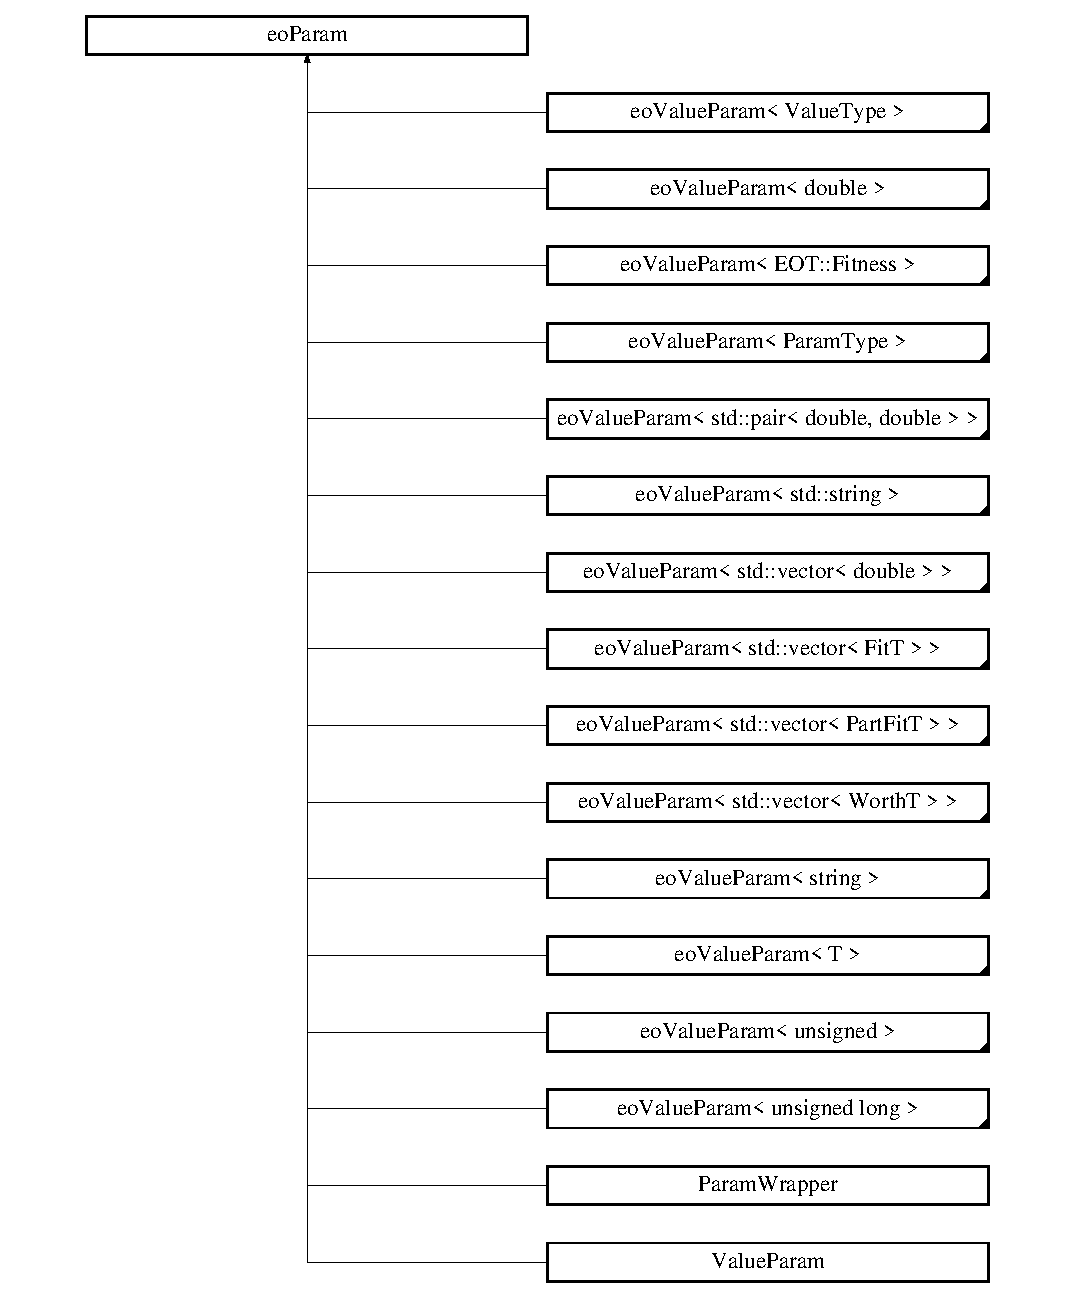
\includegraphics[height=12cm]{classeo_param}
\end{center}
\end{figure}
\subsection*{Public Member Functions}
\begin{CompactItemize}
\item 
{\bf eo\-Param} ()\label{classeo_param_a0}

\begin{CompactList}\small\item\em Empty constructor - called from outside any parser. \item\end{CompactList}\item 
{\bf eo\-Param} (std::string \_\-long\-Name, std::string \_\-default, std::string \_\-description, char \_\-short\-Name=0, bool \_\-required=false)
\begin{CompactList}\small\item\em Construct a Param. \item\end{CompactList}\item 
virtual {\bf $\sim$eo\-Param} ()\label{classeo_param_a2}

\begin{CompactList}\small\item\em Virtual destructor is needed. \item\end{CompactList}\item 
virtual std::string {\bf get\-Value} () const =0\label{classeo_param_a3}

\begin{CompactList}\small\item\em Pure virtual function to get the value out. \item\end{CompactList}\item 
virtual void {\bf set\-Value} (const std::string \&\_\-value)=0\label{classeo_param_a4}

\begin{CompactList}\small\item\em Pure virtual function to set the value. \item\end{CompactList}\item 
char {\bf short\-Name} () const \label{classeo_param_a5}

\begin{CompactList}\small\item\em Returns the short name. \item\end{CompactList}\item 
const std::string \& {\bf long\-Name} () const \label{classeo_param_a6}

\begin{CompactList}\small\item\em Returns the long name. \item\end{CompactList}\item 
const std::string \& {\bf description} () const \label{classeo_param_a7}

\begin{CompactList}\small\item\em Returns the description of the argument. \item\end{CompactList}\item 
const std::string \& {\bf def\-Value} () const \label{classeo_param_a8}

\begin{CompactList}\small\item\em Returns the default value of the argument. \item\end{CompactList}\item 
void {\bf def\-Value} (const std::string \&str)\label{classeo_param_a9}

\begin{CompactList}\small\item\em Sets the default value of the argument,. \item\end{CompactList}\item 
void {\bf set\-Long\-Name} (std::string \_\-long\-Name)\label{classeo_param_a10}

\begin{CompactList}\small\item\em ALlows to change the name (see the prefix in {\bf eo\-Parser.h}{\rm (p.\,\pageref{eo_parser_8h})}). \item\end{CompactList}\item 
bool {\bf required} () const \label{classeo_param_a11}

\begin{CompactList}\small\item\em Returns if required or not. \item\end{CompactList}\end{CompactItemize}
\subsection*{Private Attributes}
\begin{CompactItemize}
\item 
std::string {\bf rep\-Long\-Name}\label{classeo_param_r0}

\item 
std::string {\bf rep\-Default}\label{classeo_param_r1}

\item 
std::string {\bf rep\-Description}\label{classeo_param_r2}

\item 
char {\bf rep\-Short\-Hand}\label{classeo_param_r3}

\item 
bool {\bf rep\-Required}\label{classeo_param_r4}

\end{CompactItemize}


\subsection{Detailed Description}
eo\-Param: Base class for monitoring and parsing parameters 



Definition at line 42 of file eo\-Param.h.

\subsection{Constructor \& Destructor Documentation}
\index{eoParam@{eo\-Param}!eoParam@{eoParam}}
\index{eoParam@{eoParam}!eoParam@{eo\-Param}}
\subsubsection{\setlength{\rightskip}{0pt plus 5cm}eo\-Param::eo\-Param (std::string {\em \_\-long\-Name}, std::string {\em \_\-default}, std::string {\em \_\-description}, char {\em \_\-short\-Name} = {\tt 0}, bool {\em \_\-required} = {\tt false})\hspace{0.3cm}{\tt  [inline]}}\label{classeo_param_a1}


Construct a Param. 

\begin{Desc}
\item[Parameters:]
\begin{description}
\item[{\em \_\-long\-Name}]Long name of the argument \item[{\em \_\-default}]The default value \item[{\em \_\-description}]Description of the parameter. What is useful for. \item[{\em \_\-short\-Name}]Short name of the argument (Optional) \item[{\em \_\-required}]If it is a necessary parameter or not \end{description}
\end{Desc}


Definition at line 60 of file eo\-Param.h.

The documentation for this class was generated from the following file:\begin{CompactItemize}
\item 
eo\-Param.h\end{CompactItemize}
